\chapter{Related Work}\label{ch:related-work}

\lettrine{\textcolor{accent_color}{A}}{s} the fields of \acrlong{vsn} and \acrshort{rl} are very broad, this chapter aims to provide an extensive and organized overview of the most relevant works in the literature.
More specifically, this chapter delves into the main topics discussed alongside this thesis.
Since the main focus of this thesis is within robotic navigation, \acrshort{vsn} is the first topic covered.
It will lay the groundwork for how the other topics are related to robotic navigation and how they can be applied.
The following section will cover the sparsity and exploration methods, which are crucial for addressing the challenges of sparse rewards and exploration in \acrshort{rl}.
The next section will discuss the simulation-to-reality transfer in robotic navigation, which is essential for deploying models trained in simulation to real robots.
The subsequent section will cover offline \acrshort{rl}, which is a paradigm that allows training models using fixed datasets, without the need for online data collection.
Finally, the last section will discuss meta \acrshort{rl}, which focuses on learning policies that can quickly adapt to new environments.

While section~\ref{sec:visual-semantic-navigation} applies to the whole content of this document, the rest of the sections are more focused on the specific contributions of this thesis:

\begin{itemize}
    \item Section~\ref{sec:sparsity-and-exploration-methods} refers to chapter~\ref{ch:understanding-robotic-visual-semantic-navigation}, which explores exploration methods based on the use of procedural environments and simulated environments.
    \item Section~\ref{sec:simulation-to-reality-transfer-in-robotic-navigation} is related to chapter~\ref{ch:ros4vsn:-enable-real-world-robotic-visual-semantic-navigation}, which presents the ROS4VSN library, allowing the integration of different \acrshort{vsn} models in real robots.
    \item Section~\ref{sec:offline-reinforcement-learning} is related to chapter~\ref{sec:offline_rl4rvsn}, which explores the use of offline \acrshort{rl} techniques to train navigation policies in simulated environments.
    \item Section~\ref{sec:meta-imitation-learning} is related to chapter~\ref{sec:mil-for-real-world-navigation}, which explores the use of meta-imitation learning techniques to train navigation policies that can quickly adapt to new environments.
\end{itemize}

\section{Visual Semantic Navigation}\label{sec:visual-semantic-navigation}

\acrfull{vsn} is a subfield of robotic navigation that focuses on enabling robots to navigate in environments using visual observations and semantic information.
In this context, semantic information refers to the understanding of the environment's objects and their relationships, which can be used to guide the robot's navigation decisions.
\acrshort{vsn} algorithms can be categorized into different approaches based on their training methods and architectures.
For the sake of clarity, this document follows the same categorization as~\cite{gervet2022}, depicted in the figure~\ref{fig:vsn-categories}.
This classification separates the approaches into three main categories: classical methods, modular-learning-based methods and end-to-end learning methods.

\begin{figure}
    \centering
    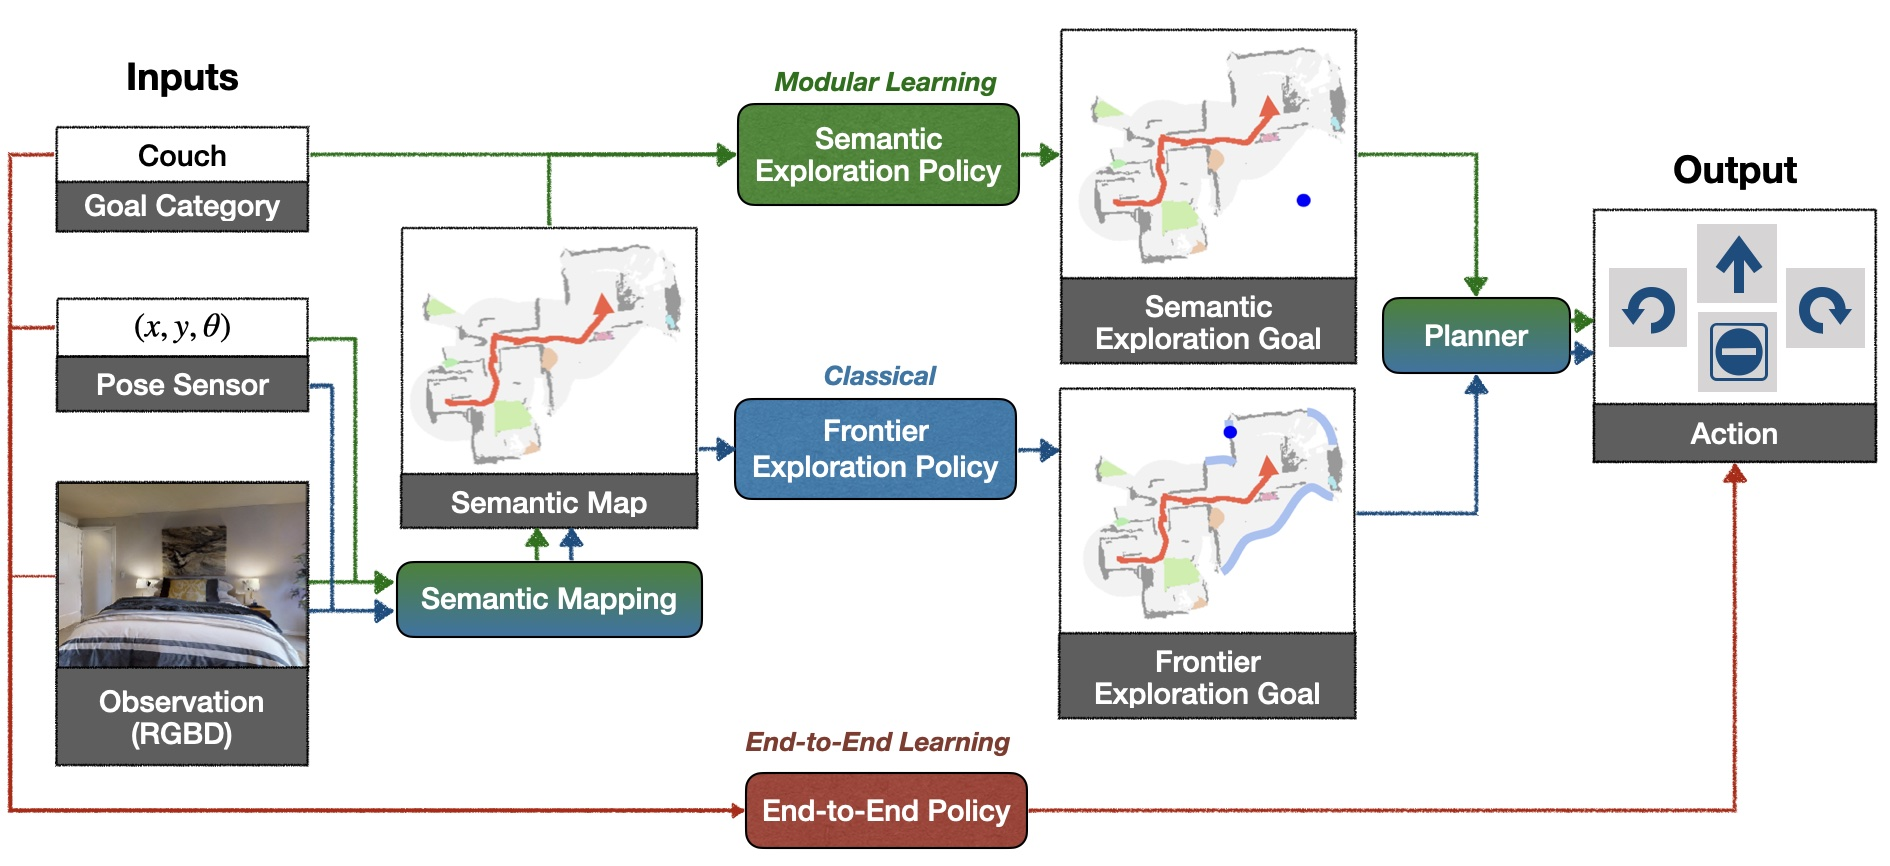
\includegraphics[width=\textwidth]{figures/related_work/methods_overview}
    \caption[Methods for \acrlong{vsn}]{When navigating via visual observations, several approaches can be taken.
    Classical methods rely on geometrical approaches to map the environment and explore it.
    Modular-learning methods use different modules to decompose the navigation problem into smaller tasks, such as exploration and navigation.
    End-to-end learning methods use deep neural networks to learn the navigation policy directly from visual observations.
    Figure from \cite{gervet2022}.}
    \label{fig:vsn-categories}
\end{figure}

\subsection{Classical methods}\label{subsec:classical-methods}

To navigate in unfamiliar environments, traditional methods use depth sensors~\cite{newcombe2011, thrun2001} and RGB cameras~\cite{jones2011, sattler2018} to build geometric maps and simultaneously determine the robot's position in relation to the map.
This is known as \acrfull{slam}~\cite{Kazerouni2022, campos2021, labbe2022}).
Typically, these \acrshort{slam} models use heuristic algorithms to create graph-based representations of the environment, allowing the robot to visit the different nodes of the graph when navigating to specific points.
Semantic \acrshort{slam} (\eg~\cite{zhang2018, jin2023}) expands upon \acrshort{slam} by integrating semantic data from the environment, allowing the robot to identify and store objects in memory.
One of the most well-known approaches in this category is the Kimera system~\cite{rosinol2020} (see figure \ref{fig:kimera-chart}), which uses a modular architecture to combine different modules for visual odometry, semantic segmentation, and object detection.

\begin{figure}
    \centering
    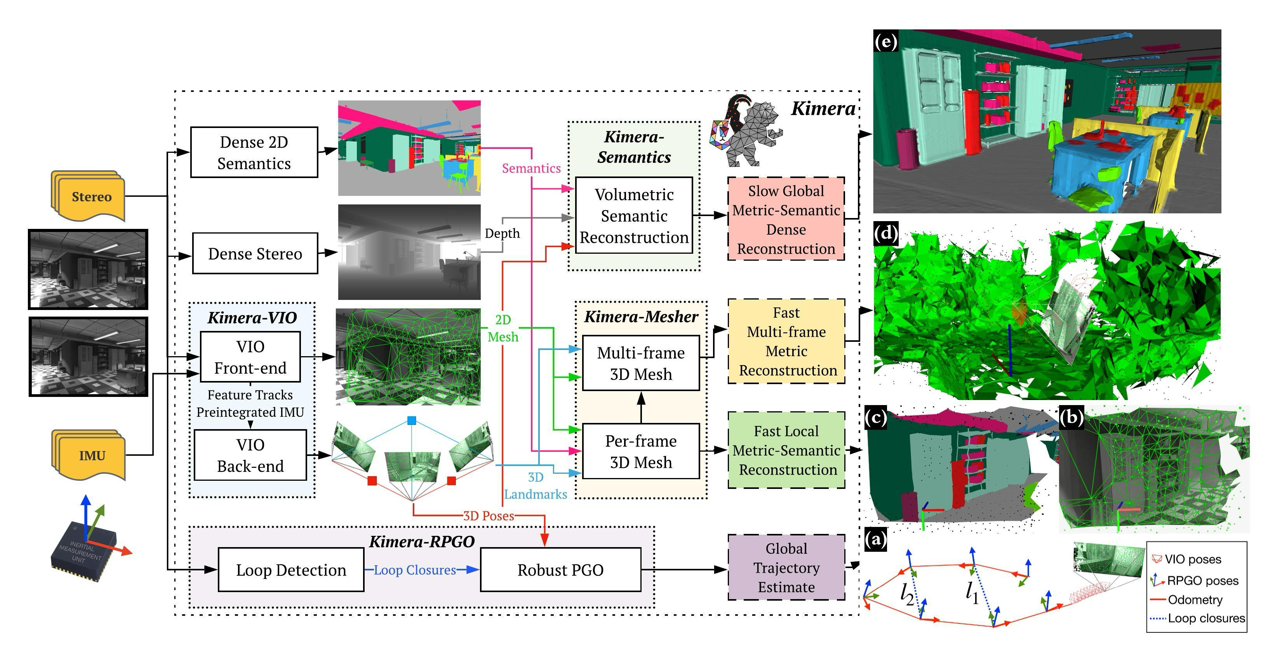
\includegraphics[width=\textwidth]{figures/related_work/kimera_chart_25 Large}
    \caption[Kimera method for semantic \acrshort{slam}]{Kimera method is one of the most representative in the semantic \acrshort{slam} category.
    It uses a modular architecture to combine different modules for images and \acrfull{imu} data, outputting pose estimations (a) and multiple metric-semantic reconstructions (b-e).
    Figure from~\cite{rosinol2020}.}
    \label{fig:kimera-chart}
\end{figure}

\subsection{Modular-learning-based methods}\label{subsec:modular-learning-based-methods}

Modular-learning-based approaches~\cite{chaplot2020, chang2020, skillfusion, Li2023RDDRLAR, zhou2022improving, Cai2024DGMemLV, Wang2023ProbableOL, Wasserman2023ExploitationGuidedEF, Yokoyama2023VLFMVF} decompose the navigation process in separate modules that execute different tasks.
It is common for these methods to be composed of a high-level semantic exploration module trained by \acrshort{RL} that indicates the agent subgoals that have to be reached by a low-level navigation policy.
One of the best examples of modularity in \acrshort{vsn} is the Hierarchical Scene Priors NAVigation (HSPNav)~\cite{Kang2024HSPNavHS}, which is shown in the figure~\ref{fig:modular-learning}.
HSPNav is a highly modular approach that uses Local and Global Scene Priors to build a semantic understanding of the environment, which then is used by a \acrshort{dqn}-based~\cite{mnih2013} navigation policy to navigate to the specified goal.
Modular learning can be also combined with offline \acrshort{rl}~\cite{shah2022} techniques to leverage navigation behaviors from fixed datasets, without any additional online data collection or fine-tuning.

\begin{figure}
    \centering
    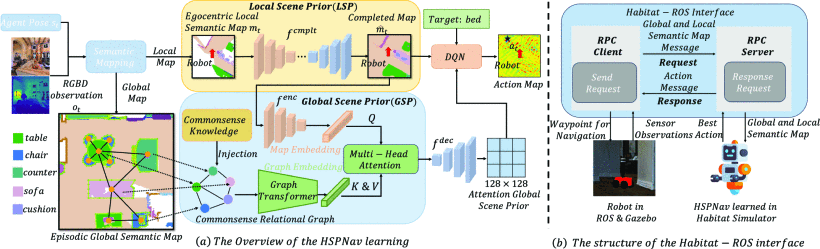
\includegraphics[width=\textwidth]{figures/related_work/modular_learning}
    \caption[Hierarchical Scene Priors NAVigation (HSPNav) for \acrlong{vsn}]{\textbf{Hierarchical Scene Priors NAVigation (HSPNav)} for \acrlong{vsn}.
    This modular-learning-based approach decomposes the navigation learning (a) into several modules:
    A semantic mapping module is used to build a semantic map of the environment, which then is further processed by an Local Scene Prior (LSP) module to refine semantically a local map.
    A topological global graph is built at the same time as a Global Scene Prior (GSP).
    These both modules are then fed into a \acrshort{dqn}-based navigation policy that outputs the next action to be executed by the robot.
    It also includes a module built on top of RPC (b) to bridge the gap between Habitat simulator and \acrshort{ros}, allowing the use of the Habitat-trained policies to be refined on Gazebo simulator.
    Figure from~\cite{Kang2024HSPNavHS}.}
    \label{fig:modular-learning}
\end{figure}

\subsection{End-to-end learning methods}\label{subsec:end-to-end-learning-methods}

A recent approach, made possible by advances in machine learning and computer vision, involves designing navigation policies that directly train deep neural networks to learn semantic information from visual observations in an end-to-end fashion (\eg~\cite{ramrakhya2022, yadav2022, gutierrez2019, khandelwal2022, chaplot2020,chang2020}).
This approach is termed \acrlong{vsn}.
These models often rely on the use of \acrshort{cnn}s as visual encoders followed by \acrshort{rnn}s; that are in charge of predicting an action distribution directly from raw input observations.
The neural networks are trained using \acrfull{il} or \acrshort{rl} approaches.

When \acrshort{il} is applied to the visual navigation problem, navigation policies are learnt from expert demonstrations (\eg~\cite{ramrakhya2022,yadav2022}).
It can also be used combined with a \acrshort{rl} fine-tuning phase to achieve better performance~\cite{ramrakhya2023}.

Other works focus on the use of an end-to-end \acrshort{rl} approach to solve \acrfull{objnav} navigation~\cite{zhu2017, gutierrez2019, khandelwal2022, Liu2022, Yadav2023OVRLV2AS, Xu2024DeepRL, YokoyamaHM3DOVONAD}.
One of the most notable examples is the \acrfull{ddppo}~\cite{wijmans2020}, which laid the foundation and framework for training end-to-end and modular learning agents within Habitat simulator.
\acrshort{ddppo} uses a \acrfull{ppo}~\cite{schulman2017} algorithm to train a visual navigation policy that can navigate to specified goals in a simulated environment.
It also does it via Synchronous-\acrshort{rl} (see figure \ref{fig:ddppo}), which allows the agent to learn from multiple GPU batched environments, speeding up the training process.
Some authors have proposed combining the \acrshort{rl} training with different strategies, like auxiliary tasks~\cite{ye2021}, improved visual representations via object relation graphs~\cite{yang2018}, semantic segmentations~,\cite{Mousavian2018} or combining audio feedback with the visual inputs~\cite{Wang2023, Kondoh2023MultigoalAN}.

\begin{figure}
    \centering
    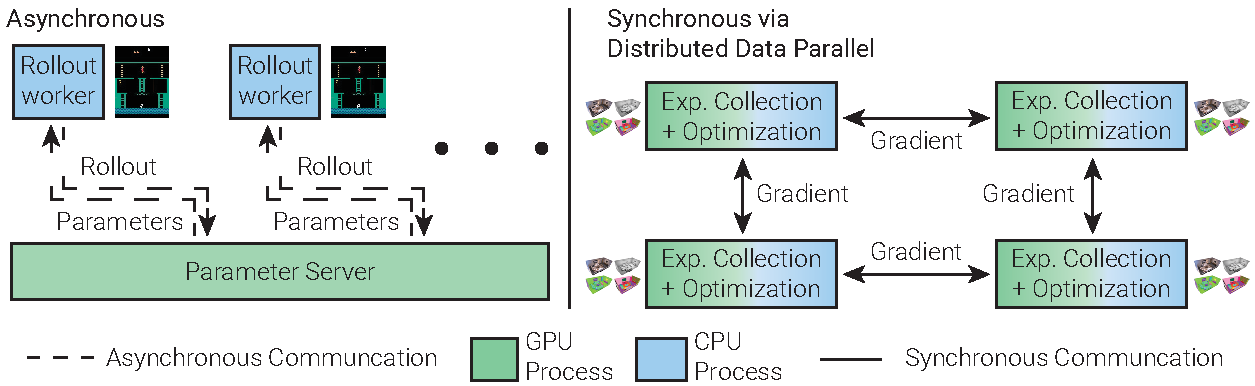
\includegraphics[width=\textwidth]{figures/related_work/ddppo}
    \caption[Decentralized Distributed Proximal Policy Optimization (DD-PPO)]{\textbf{Decentralized Distributed Proximal Policy Optimization (DD-PPO)}.
    This algorithm is included in the Habitat Lab as a baseline for training end-to-end visual navigation policies.
    It laid the foundation for the majority of the subsequent works in the field and it is used in this thesis as well.
    While typical \acrshort{rl} has been trained in an asynchronous manner, \acrshort{ddppo} uses a synchronous approach to train the agent in multiple environments at the same time.
    Figure from~\cite{wijmans2020}.}
    \label{fig:ddppo}
\end{figure}

Finally, there are different approaches that try to tackle the problem of rapidly adapting to unseen environments in visual navigation via meta-learning~\cite{wortsman2019, luo2021, zhang2022}.
These methods are trained on a variety of different environments (usually designated as tasks) and are able to generalize to unseen environments by learning a policy that can be quickly adapted to new environments.
And the recent progress in large language models (LLMs) has led to the possibility of using them to solve the visual navigation problem~\cite{Huang2023, Zhou2023} as well.
In this case, the LLMs are used as a reasoning module in charge of understanding the semantic information present on the environment.
They then share this information with different modules in charge of navigating to the specified goal.

This work focuses on the end-to-end learning-based methods, specifically on the analysis of the behavior of these models in the real world and the use of \acrshort{rl} and \acrshort{il} techniques to train visual navigation policies in simulated environments.

\section{Sparsity and exploration methods}\label{sec:sparsity-and-exploration-methods}
To address the sparse reward and exploration problems, different approaches have been proposed.
Auxiliary tasks~\cite{jaderberg2016, ye2021} help the agent to explore the environment and gather extrinsic reward by maximizing pseudo-reward functions.
Curiosity-driven exploration~\cite{pathak2017} (depicted on figure \ref{fig:curiosity}) leverages on the error of the agent's ability to predict the next state to introduce a new intrinsic reward that enables the agent to explore the environment.
When dealing with procedurally generated environments, a curriculum learning mechanism can be incorporated so the episodes are ordered by an exploration score~\cite{zha2020b}, and then the agent imitates the best ones.
This thesis, in chapter~\ref{ch:understanding-robotic-visual-semantic-navigation}, also uses procedurally generated environments, but it relies on a \acrshort{rl} approach combined with reward shaping~\cite{ng1999, jestel2021} and $\epsilon\text{-}greedy$~\cite{mnih2013} techniques to learn to navigate in them.

\begin{figure}
    \centering
    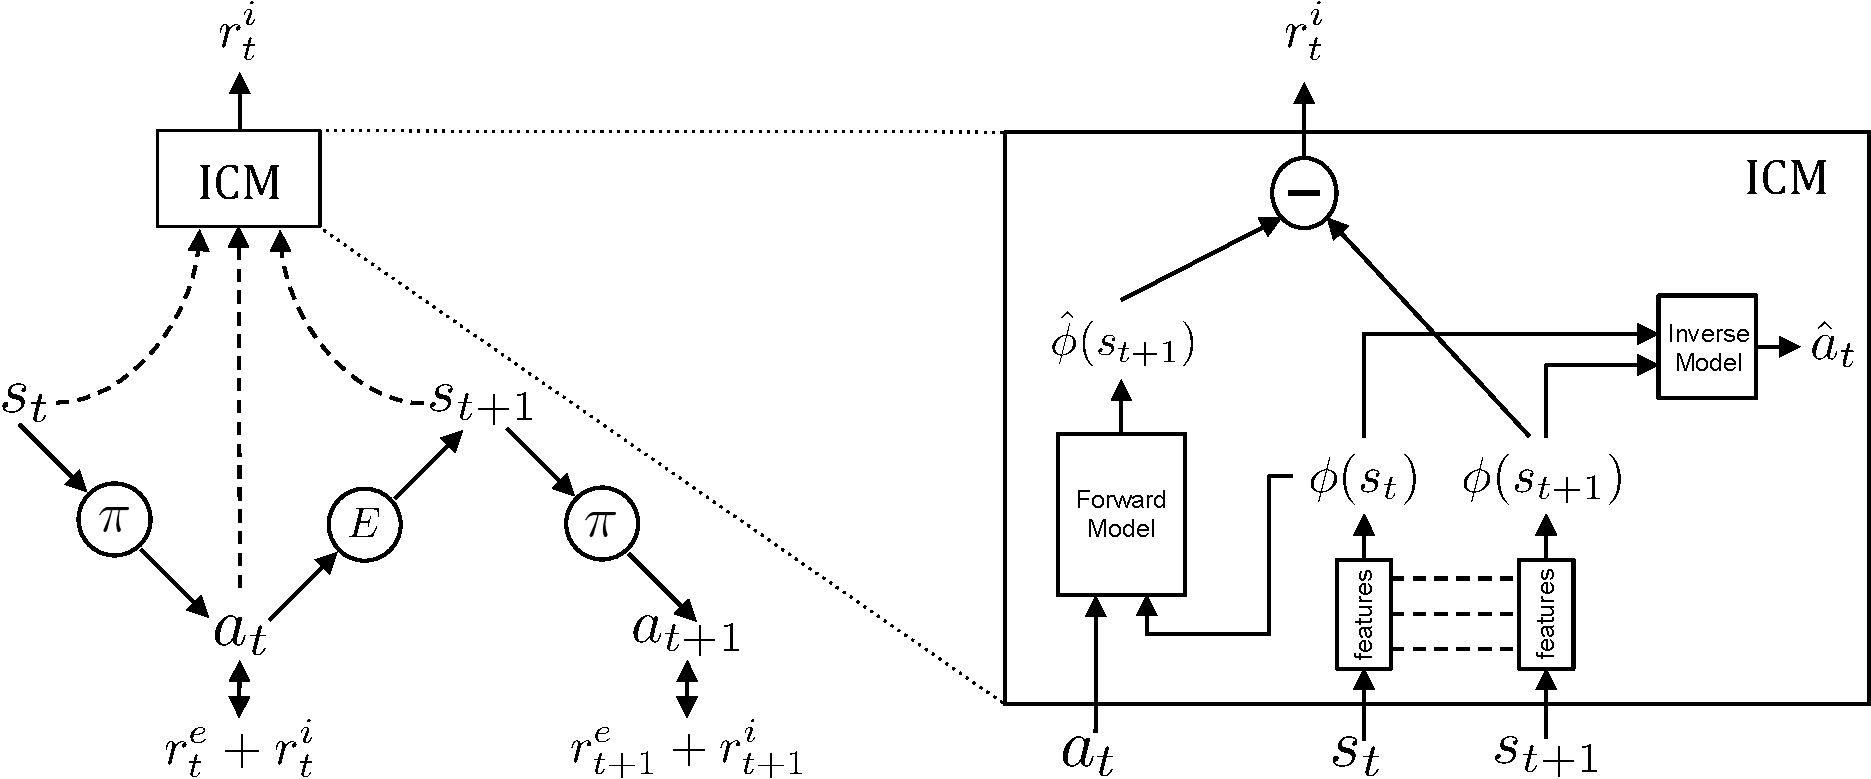
\includegraphics[width=\textwidth]{figures/related_work/curiosity}
    \caption[Curiosity-driven exploration]{\textbf{Curiosity-driven exploration} is a technique that uses the error of the agent's ability to predict the next state to introduce a new intrinsic reward that enables the agent to explore the environment.
    The agent learns a forward model that predicts the next state given the current state and action.
    The intrinsic reward is then computed as the error between the predicted and actual next state.
    Figure from~\cite{pathak2017}.}
    \label{fig:curiosity}
\end{figure}

\section{Simulation-to-reality transfer in robotic navigation}\label{sec:simulation-to-reality-transfer-in-robotic-navigation}
Deploying a model trained in simulation to a real robot is a challenging task.
Due to logistical constraints, training a model in the real world —especially with \acrshort{rl} techniques— is often impractical, prompting the use of alternative methods to address this challenge.
For example,~\cite{kim2022} proposes a monocular vision-based time-to-collision estimation for small drones by domain adaptation of simulated images.
Their method converts simulated images into real-like synthetic images using a sim-to-real method.
This is done with the aim of minimizing efforts and time invested in the collection of training datasets within real-world scenarios, while simultaneously maximizing the advantages inherent in simulated environments.

Overall, it is necessary to develop methods that allow efficiently transfer the knowledge learnt in simulation to the real world.
Different approaches have been proposed to solve this problem.
In ~\cite{kadian2020}, an exact replica of a real scenario is simulated (see figure~\ref{fig:sim2real}).
This allows the authors to explore the behavior of visual navigation policies both in simulation and in reality and how their performance correlates.
For instance, CAD2RL~\cite{sadeghiCAD2RLRealSingleImage2017} system achieved remarkable success in training a collision avoidance policy entirely within a simulated environment.
This breakthrough was subsequently tested on real aerial drones, with promising results.
By focusing on simulation refinement~\cite{Son2020}, the accuracy of simulations can be improved by exploiting the disparities between simulated and real-world observations.
In the field of locomotion, training legged robotic systems in a simulated environment and subsequently transferring the acquired policies to real-world applications~\cite{Hwangbo_2019, agarwal2022} have always been a challenging task.

\begin{figure}
    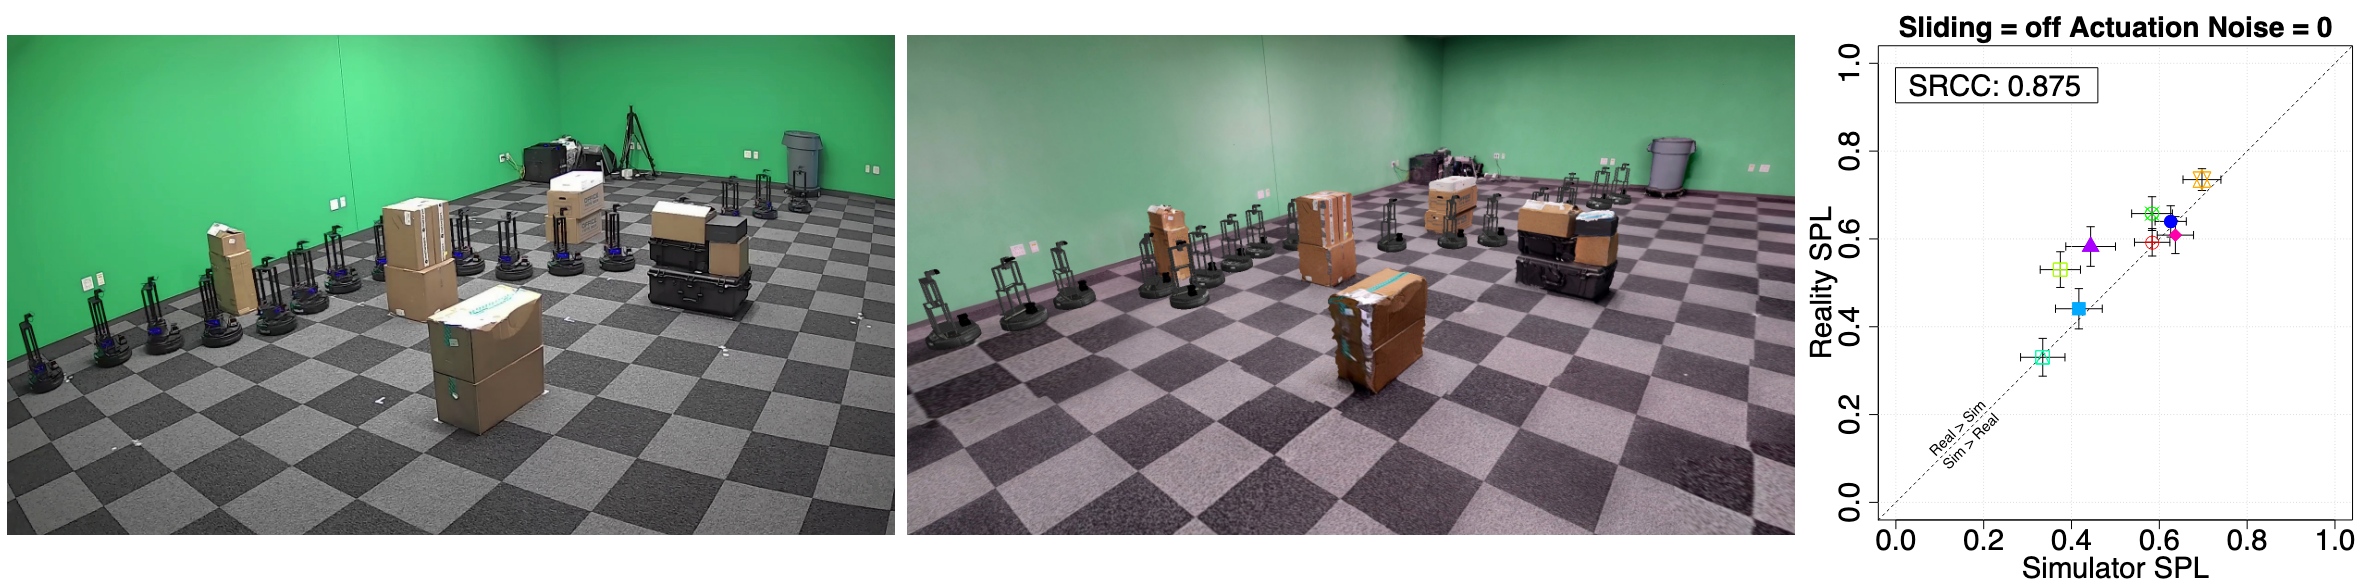
\includegraphics[width=\textwidth]{figures/related_work/sim2real}
    \caption[Simulation-to-reality transfer]{\textbf{Simulation-to-reality transfer} is a challenging task in robotic navigation.
    In this example, a real-world scenario is simulated to explore the behavior of visual navigation policies both in simulation and in reality.
    The authors use a simulated environment that closely resembles the real-world scenario, allowing them to train and evaluate their policies in a controlled setting.
    Figure from~\cite{kadian2020}.}
    \label{fig:sim2real}
\end{figure}

For the problem of \acrshort{vsn}, the study by~\cite{gervet2022} shows how different approaches behave in real-world settings.
They compare the performance of different \acrshort{vsn} methods in simulated and real-world environments, concluding that modular-learning approaches outperform end-to-end learning methods in real-world scenarios.
Interestingly, the conclusion of chapter~\ref{ch:ros4vsn:-enable-real-world-robotic-visual-semantic-navigation}, is the same as in~\cite{gervet2022}: that modular-learning approaches are the best ones for deployment in the real world.

\section{Offline Reinforcement Learning}\label{sec:offline-reinforcement-learning}

Offline reinforcement learning (offline \acrshort{rl}) refers to learning a policy from a fixed dataset of environment interactions, without additional online exploration~\cite{levine2020} (figure \ref{fig:diagram-offline}).
This paradigm is appealing for robotics, where collecting data is costly or risky, since it allows agents to leverage large logs of prior experiments or demonstrations.
However, a core challenge in offline \acrshort{rl} is distributional shift: the learned policy may choose state-action pairs not well-covered by the dataset, leading to arbitrarily bad value estimates and unstable policy updates.
Over the past years, a number of algorithmic strategies have been proposed to address this issue and enable effective offline learning of robotic skills.

\begin{figure}
    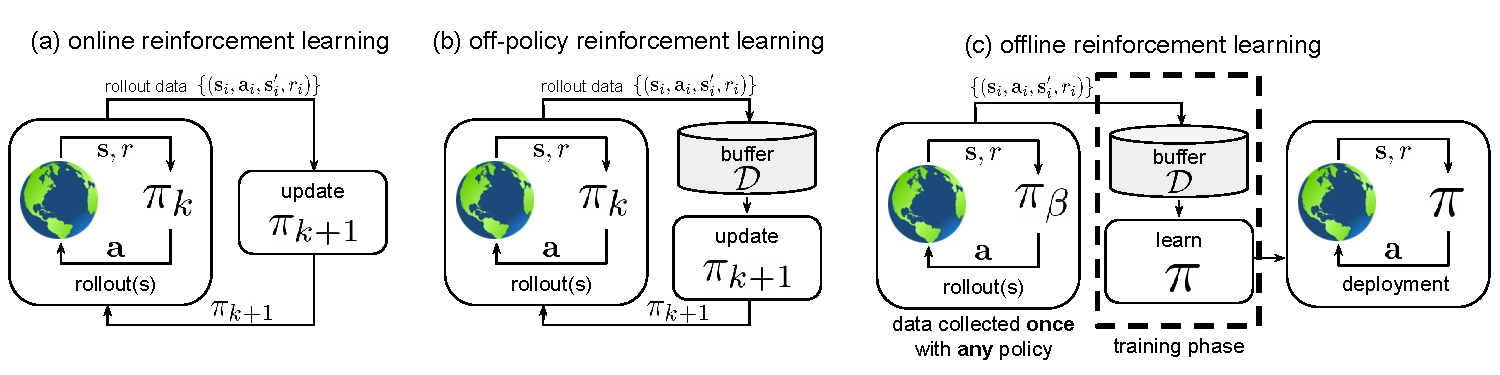
\includegraphics[width=\textwidth]{figures/related_work/diagram_offline}
    \caption[Offline reinforcement learning paradigm]{\textbf{Offline reinforcement learning} is a paradigm that allows training models using fixed datasets, without the need for online data collection.
    In this diagram, the offline RL process is depicted, where a dataset of environment interactions is used to train a policy.
    The policy is then evaluated in the environment, and the process is repeated until convergence.
    Figure from~\cite{levine2020}.}
    \label{fig:diagram-offline}
\end{figure}

\subsection{Conservative Value Estimation}\label{subsec:conservative-value-estimation}

One line of work imposes \textit{pessimism} in value function learning to avoid overestimating unseen actions.
For example, Conservative Q-Learning (CQL)~\cite{conservative} augments the Bellman objective with a penalty on Q-values for out-of-distribution actions.
By learning a deliberately conservative Q-function (lower-bounding the true values), CQL prevents the policy from exploiting spurious high rewards for actions outside the dataset support.
Similarly, \acrfull{iql}~\cite{kostrikov2022offline} avoids querying unseen actions altogether during training.
Instead of a max over actions, \acrshort{iql} uses an expectile regression to estimate the value of the \textit{best} in-dataset actions, then extracts a policy via advantage-weighted behavior cloning.

\subsection{Policy Constraints and Behavior Regularization}\label{subsec:policy-constraints-and-behavior-regularization}

Another broad strategy is to constrain the learned policy to stay close to the behavior policy that generated the data.
A prominent example is Batch-Constrained deep Q-learning (BCQ)~\cite{Fujimoto2018OffPolicyDR}, which modifies the Q-learning update to consider only actions that are likely under the offline dataset instead of maximizing over all actions.
In practice, BCQ trains a generative model (e.g.,\ a \acrfull{vae}) to produce candidate actions similar to those in the dataset, ensuring that the policy cannot stray far from logged behavior.
Likewise, Bootstrapping Error Accumulation Reduction (BEAR)~\cite{Kumar2019StabilizingOQ} and Behavior-Regularized Actor-Critic (BRAC)~\cite{Wu2019BehaviorRO} add explicit divergence penalties (\eg \acrfull{kl} or \acrfull{mmd}) to keep the learned policy distribution close to the dataset behavior policy.
By limiting policy deviation, these methods address bootstrapping error and distribution shift, effectively preventing the agent from choosing out-of-distribution actions with erroneously high value estimates.
Variants of this idea combine \acrshort{rl} updates with imitation learning: for instance, Advantage-Weighted Actor-Critic (AWAC)~\cite{Nair2020AcceleratingOR} and Critic-regularized Regression (CRR)~\cite{NEURIPS2020_588cb956} constrain the policy toward the dataset behavior while weighting actions by their estimated advantages, thus improving performance without sacrificing stability.
Overall, policy constraint and behavior regularization approaches have proven effective both in simulation and in real-world settings by leveraging the data’s demonstrated behaviors as an anchor.

The work presented in chapter~\ref{sec:offline_rl4rvsn} builds upon these ideas, using a modified version of \acrshort{iql}~\cite{kostrikov2022offline} to train a navigation policy from a fixed dataset of demonstrations.

\section{Few-Shot Meta-Imitation Learning}\label{sec:meta-imitation-learning}

\acrfull{mil} extends imitation learning into the meta-learning regime, allowing robots to rapidly learn new skills from only a few demonstrations by leveraging experience across many tasks.
The core idea is to extract common knowledge or a prior policy from a distribution of training tasks, such that only minimal adaptation is needed to master a new task.
Early works demonstrated one-shot imitation of robotic manipulation tasks by meta-training over multiple demonstrations~\cite{Duan2017OneShotIL, finnOneShotVisualImitation2017}.
Depending on the method used, three main approaches can be distinguished: gradient-based and contextual and latent variable meta-imitation learning.

\subsection{Gradient-based Meta Imitation Learning}\label{subsec:gradient-based-meta-imitation-learning}

Many subsequent \acrshort{mil} approaches have adopted gradient-based adaptation for fast imitation.
In these methods, a policy (or policy initialization) is meta-learned such that a small number of gradient steps on a new task’s demo data leads to effective behavior cloning on that task.
For example, \acrfull{maml}~\cite{finn2017} learns a policy initialization that can be quickly adapted to new tasks via gradient descent.
The idea is to find the optimal parameters $\theta$ over a distribution of tasks $\mathcal{D}$ such that a few gradient steps on the task-specific data $\mathcal{D}_i$ lead to good performance on the task reward $R_i$ (see figure~\ref{fig:maml-mil}).

\acrshort{maml} is specifically designed for reinforcement and supervised learning, but it can also be applied to behavior cloning losses, yielding one-shot imitation learners for robot manipulation and locomotion domains.
The meta-learned policy serves as a strong prior that encodes behaviors common to all training tasks, and adaptation fine-tunes this prior to the specifics of the new task.
Previous works have extended \acrshort{maml} to the context of imitation learning, such as learning from video demonstrations of robotic tasks~\cite{finnOneShotVisualImitation2017} or learning from human demonstrations in complex environments~\cite{Yu2018OneShotIF}.
Figure~\ref{fig:maml-mil} illustrates the whole idea of gradient-based meta-imitation learning applied to a real use case of robotic manipulation, where the agent learns to recognize and push a new object from a single human demonstration.

% add a two column subfigure
\begin{figure}
    % subfigure a
    \centering
   \begin{subfigure}[b]{0.49\linewidth}
        \centering
        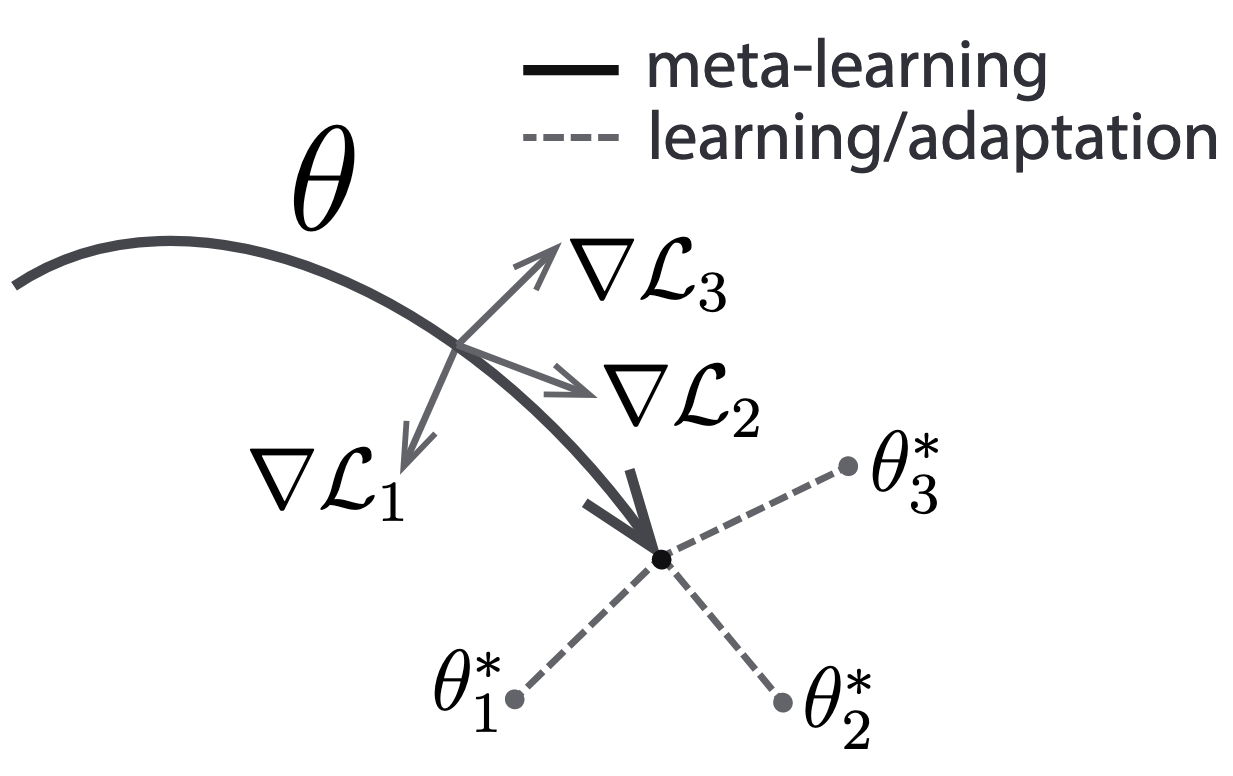
\includegraphics[width=\linewidth]{figures/related_work/maml}
        \caption{Diagram of \acrfull{maml}.}
        \label{fig:maml}
    \end{subfigure}
    \hfill
    \begin{subfigure}[b]{0.49\linewidth}
        \centering
        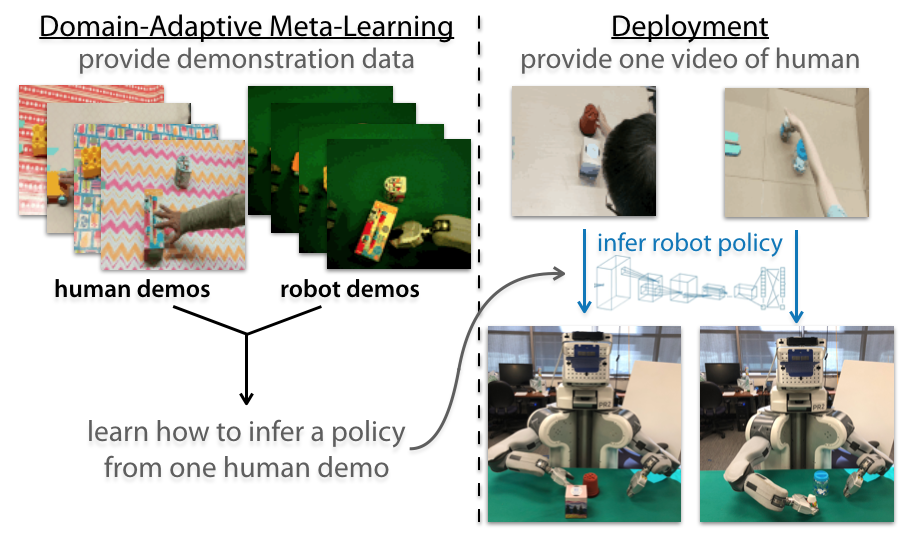
\includegraphics[width=\linewidth]{figures/related_work/one_shot_human}
        \caption{The idea behind one-shot imitation learning.}
        \label{fig:oneshot-human}
    \end{subfigure}
    \caption[Gradient-based meta-imitation learning]{\textbf{Gradient-based meta-imitation learning} is a technique that learns a policy initialization that can be quickly adapted to new tasks via gradient descent.
    On \ref{fig:maml}, the meta-learning process is depicted, where a policy initialization $\theta$ is optimized over a distribution of tasks $\mathcal{D}$.
    On \ref{fig:oneshot-human}, a whole process of one-shot imitation learning is shown.
    The agent is meta-trained on a distribution of human and robot demonstration data.
    Then, it learns to recognize and push a new object from a single human demonstration.
    Figures from~\cite{finn2017} and \cite{Yu2018OneShotIF} respectively.}
    \label{fig:maml-mil}
\end{figure}

Several recent works have built upon \acrshort{maml} to improve its efficiency and applicability to more complex imitation tasks.
Dual Meta Imitation Learning (DMIL)~\cite{gao2022transferring} proposes a hierarchical meta-imitation learning framework that learns both a high-level policy and a low-level subskills controller via \acrshort{maml}.
Meta-Imitation Learning with Adaptive Dynamical Primitives (MiLa)~\cite{Wu2024OneShotRI} allows for learning to new tasks via a single unsegmented long-horizon demonstration.

\subsection{Contextual and Latent Variable Meta-Imitation}\label{subsec:contextual-and-latent-variable-meta-imitation}

An alternative line of work avoids explicit gradient updates at test time by conditioning the policy on task-specific context, typically derived from demonstrations.
Instead of learning an initial set of weights for all tasks, these methods learn to encode demonstrations into a latent representation that informs the policy of the current task.
Typically, one-shot imitation learning models process a demonstration trajectory (or a few demos) through an encoder – using architectures like recurrent networks or self-attention – and feed this context alongside the current state to the policy network~\cite{Duan2017OneShotIL}.
The policy thus “infers” the intended task from the demo and executes the corresponding behavior, without needing gradient fine-tuning on the new task.
Another instantiation of this idea is to use latent variables~\cite{sontakke2023roboclip, NEURIPS2019_2b8f621e, NEURIPS2019_30de2428, 10.3389/frobt.2020.606361, Bhoopchand2023LearningFI} to represent tasks: during meta-training, a latent context $z$ is inferred for each demonstration set (via, say, a variational encoder or recurrent inference), and the policy or value function is conditioned on $z$ rather than relying on one global initialization.
This approach, inspired by contextual meta-\acrshort{rl}, addresses the limitation of a single meta-parameter set by allowing task-specific adaptation in the latent space.
For instance, figure~\ref{fig:transformer-mil} shows how task representations can be encoded into parametrized state encoders using transformers~\cite{cho2024metacontroller}.

\begin{figure}
    \centering
    \includegraphics[width=\textwidth]{figures/related_work/transformer_mil}
    \caption[Meta-Controller]{\textbf{Meta-Controller}: a technique for few-shot imitation learning to simultaneously generalize to unseen embodiments and tasks using a few demonstrations.
    First, the states and actions are encoded into a sequence of joint-level tokens.
    Then, these state tokens are encoded by the state encoder to obtain a task representation.
    Finally, the task representation is used to condition the matching-based policy network, which outputs the next action to be executed by the robot.
    Figure from~\cite{cho2024metacontroller}.}
    \label{fig:transformer-mil}
\end{figure}

Chapter~\ref{sec:meta-imitation-learning} extends the concepts of gradient-based meta-imitation learning (section~\ref{subsec:gradient-based-meta-imitation-learning}) by implementing a modified version of \acrshort{maml}~\cite{finn2017} to train navigation policies using demonstrations in a meta-imitation learning fashion.
